\documentclass[tikz,margin=1mm]{standalone}


\begin{document}
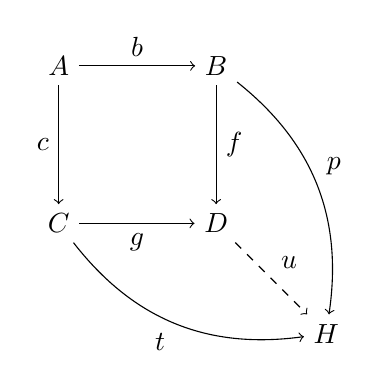
\begin{tikzpicture}[node distance=2cm, auto]
  \node (A) {$A$};
  \node[right of=A] (B) {$B$};
  \node[below of=A] (C) {$C$};
  \node[below of=B] (D) {$D$};
  \node[node distance=1.4cm, right of=D, below of=D] (H) {$H$};

  \draw[->] (A) to node{$b$} (B);
  \draw[->] (A) to node[swap]{$c$} (C);
  \draw[->] (B) to node{$f$} (D);
  \draw[->] (C) to node[swap]{$g$} (D);

  \draw[->, bend left ] (B) to node{$p$} (H);
  \draw[->, bend right] (C) to node[swap]{$t$} (H);

  \draw[->, dashed] (D) to node{$u$} (H);

\end{tikzpicture}
\end{document}

